\documentclass[aspectratio=169,10pt]{beamer}

\usepackage{fontspec}
\usepackage{xcolor}
\usepackage{colortbl}
\usepackage{tikz}
\usetikzlibrary{arrows.meta, positioning, shapes.geometric}
\usepackage{booktabs}
\usepackage{graphicx}
\usepackage{amsmath,amssymb}
\usepackage{microtype}

% ==============================================================================
% EDITORIAL SCIENTIFIC COLOR PALETTE
% ==============================================================================
\definecolor{navy}{HTML}{183B63}         % Primary heading & structural colour
\definecolor{teal}{HTML}{299D91}         % Secondary accent: workflows, takeaways, favourable results
\definecolor{coral}{HTML}{C96B70}        % Muted coral: warnings, contrasts, limitations
\definecolor{lightgrey}{HTML}{F2F4F7}    % Subtle neutral background for panels
\definecolor{charcoal}{HTML}{30343B}     % Dark charcoal body text
\definecolor{linegrey}{HTML}{E2E8F0}     % Subtle dividing lines & table borders
\definecolor{mutedgrey}{HTML}{64748B}    % Secondary metadata & captions

% ==============================================================================
% TYPOGRAPHY: EDITORIAL HIERARCHY
% ==============================================================================
\setsansfont{Helvetica Neue}[
  BoldFont={Helvetica Neue Bold},
  ItalicFont={Helvetica Neue Italic}
]
\newfontfamily\condheading{Avenir Next Condensed}[
  BoldFont={Avenir Next Condensed Bold},
  ItalicFont={Avenir Next Condensed Italic}
]

% Base beamer settings
\setbeamercolor{normal text}{fg=charcoal,bg=white}
\setbeamercolor{background canvas}{bg=white}
\setbeamercolor{structure}{fg=navy}
\setbeamertemplate{navigation symbols}{}
\setbeamersize{text margin left=8mm, text margin right=8mm}

% Itemize customization
\setbeamertemplate{itemize items}{\textcolor{teal}{\raisebox{0.2ex}{\tiny$\blacksquare$}}}
\setbeamertemplate{itemize subitem}{\textcolor{mutedgrey}{\raisebox{0.2ex}{\tiny$\circ$}}}

% ==============================================================================
% FRAMETITLE & SUBTITLE TEMPLATE
% ==============================================================================
\setbeamertemplate{frametitle}{%
  \vspace{0.10cm}%
  {\condheading\bfseries\large\textcolor{navy}{\insertframetitle}}\par%
  \ifx\insertframesubtitle\empty\else%
    \vspace{0.02cm}%
    {\scriptsize\textcolor{mutedgrey}{\insertframesubtitle}}\par%
  \fi%
  \vspace{0.06cm}%
  {\color{linegrey}\hrule height 0.5pt}%
  \vspace{0.08cm}%
}

% ==============================================================================
% FOOTER TEMPLATE (Unobtrusive & Consistent)
% ==============================================================================
\setbeamertemplate{footline}{%
  \ifnum\thepage>1
    \begin{beamercolorbox}[wd=\paperwidth,ht=0.5pt]{footrule}
      \color{linegrey}\hrule height 0.5pt width \paperwidth
    \end{beamercolorbox}%
    \begin{beamercolorbox}[wd=\paperwidth,ht=2.6ex,dp=1.0ex,leftskip=8mm,rightskip=8mm]{footline}%
      {\tiny\textcolor{mutedgrey}{Cancer RNA-Seq Classification: Flexibility vs.\ Interpretability in $p \gg n$}}%
      \hfill%
      {\tiny\textcolor{mutedgrey}{Indian Statistical Institute}}%
      \hspace{6mm}%
      {\tiny\bfseries\textcolor{navy}{\insertframenumber{} / \inserttotalframenumber}}%
    \end{beamercolorbox}%
  \fi
}

% ==============================================================================
% CUSTOM EDITORIAL COMPONENTS
% ==============================================================================

% Takeaway banner (Restrained emphasis with teal vertical rule)
\newcommand{\takeaway}[1]{%
  \vspace{0.06cm}%
  \par\noindent%
  \tikz[baseline=0.3ex]{\fill[teal] (0,0) rectangle (0.04,0.65em);}%
  \hspace{4pt}%
  {\scriptsize\textbf{\textcolor{teal}{Takeaway:}} \textcolor{charcoal}{#1}}\par%
}

% Flat grey panel for clean grouping
\newenvironment{panel}[1][]{%
  \begin{beamercolorbox}[wd=\linewidth,sep=4pt]{panelbox}%
    \if\relax\detokenize{#1}\relax\else
      {\condheading\bfseries\footnotesize\textcolor{navy}{#1}}\par\vspace{2.5pt}%
    \fi
}{%
  \end{beamercolorbox}%
}
\setbeamercolor{panelbox}{fg=charcoal,bg=lightgrey}

% Section Divider Macro
\newcommand{\sectiondivider}[3]{%
  {
    \setbeamertemplate{footline}{}
    \begin{frame}[plain]
      \vspace*{1.8cm}
      {\footnotesize\bfseries\textcolor{teal}{SECTION #1}}\par\vspace{0.20cm}
      {\condheading\bfseries\fontsize{24}{28}\selectfont\textcolor{navy}{#2}}\par\vspace{0.25cm}
      {\color{linegrey}\hrule height 0.8pt width 0.35\textwidth}\par\vspace{0.25cm}
      {\normalsize\textcolor{mutedgrey}{#3}}
    \end{frame}
  }
}

\begin{document}

% ==============================================================================
% SLIDE 1: TITLE SLIDE (Minimalist Scientific Editorial)
% ==============================================================================
{
\setbeamertemplate{footline}{}
\begin{frame}[plain]
  \vspace*{1.2cm}
  {\scriptsize\bfseries\textcolor{teal}{INDIAN STATISTICAL INSTITUTE, KOLKATA} \;\textbar{}\; \textcolor{mutedgrey}{COURSE PROJECT: REGRESSION TECHNIQUES}}\par\vspace{0.35cm}
  
  {\condheading\bfseries\fontsize{23}{27}\selectfont\textcolor{navy}{Flexibility vs.\ Interpretability in}}\par\vspace{0.08cm}
  {\condheading\bfseries\fontsize{23}{27}\selectfont\textcolor{navy}{High-Dimensional Cancer Classification}}\par\vspace{0.25cm}
  
  {\small\textcolor{mutedgrey}{Regularized Regression, Tree Ensembles, and Neural Networks on RNA-Seq Data ($p \gg n$)}}\par\vspace{0.35cm}
  
  {\color{teal}\hrule height 1.2pt width 0.20\textwidth}\par\vspace{0.45cm}
  
  {\small\textbf{\textcolor{charcoal}{Rajveer Vora \quad \textbar{} \quad Amartya Amritanshu \quad \textbar{} \quad P.\ Sanjith Reddy}}}\par\vspace{0.12cm}
  {\footnotesize\textcolor{mutedgrey}{November 2026}}
\end{frame}
}

% ==============================================================================
% SLIDE 2: THE HIGH-DIMENSIONAL SETTING (Three-Column Explanatory)
% ==============================================================================
\begin{frame}
\frametitle{The High-Dimensional Setting: $p \gg n$ Transcriptomics}
\framesubtitle{Theoretical breakdowns and biological collinearity in bulk RNA-Seq}

\begin{columns}[T]
  \begin{column}{0.31\textwidth}
    \begin{panel}[Extreme Dimensionality]
      \begin{itemize}\itemsep=3pt
        \item \textbf{$n = 801$} patient samples across $K = 5$ cancer types.
        \item \textbf{$p = 20,531$} continuous gene expression features.
        \item Underdetermined system: features outnumber observations $25 : 1$.
      \end{itemize}
    \end{panel}
  \end{column}

  \begin{column}{0.31\textwidth}
    \begin{panel}[Singular Covariance]
      \begin{itemize}\itemsep=3pt
        \item Covariance $\mathbf{S} = \frac{1}{n-1}\mathbf{X}^T\mathbf{X} \in \mathbb{R}^{p \times p}$.
        \item $\text{rank}(\mathbf{S}) \le n - 1 = 800 \ll 20,531$.
        \item $\ge 19,730$ zero eigenvalues.
        \item \textbf{OLS and Fisher LDA fail} due to singular non-invertibility.
      \end{itemize}
    \end{panel}
  \end{column}

  \begin{column}{0.31\textwidth}
    \begin{panel}[Biological Collinearity]
      \begin{itemize}\itemsep=3pt
        \item Genes act in co-regulated pathways and transcriptional modules.
        \item Thousands of gene pairs have Pearson $|r| > 0.85$.
        \item Infinite hyperplanes achieve perfect linear training separation.
      \end{itemize}
    \end{panel}
  \end{column}
\end{columns}

\takeaway{Classical unregularized estimators fail mathematically; the challenge is identifying stable, interpretable biomarkers without overfitting.}
\end{frame}

% ==============================================================================
% SECTION 01: DATASET AND EXPLORATORY ANALYSIS
% ==============================================================================
\sectiondivider{01}{Dataset and Exploratory Analysis}{RNA-Seq distributions, variance screening, and inherent linear separability}

% ==============================================================================
% SLIDE 4: DATA PROCESSING & VARIANCE FILTERING (Three-Column Comparative)
% ==============================================================================
\begin{frame}
\frametitle{Preprocessing and Unsupervised Variance Screening}
\framesubtitle{Transforming raw read counts and filtering non-informative variation}

\begin{columns}[T]
  \begin{column}{0.31\textwidth}
    \begin{panel}[Variance Stabilization]
      \textbf{Distributional Skewness:}
      \begin{itemize}\itemsep=1.5pt
        \item Raw counts span $0$ to $10^6$.
        \item Log-transformation:
          {\scriptsize $$z_{ij} = \log_2(x_{ij} + 1)$$}
        \item Symmetrizes distributions and moderates outlier spikes.
      \end{itemize}
    \end{panel}
  \end{column}

  \begin{column}{0.31\textwidth}
    \begin{panel}[Top 1,000 Variance Rationale]
      \textbf{Three Essential Factors:}
      \begin{itemize}\itemsep=1.5pt
        \item \textbf{Noise removal}: Housekeeping genes.
        \item \textbf{Feasibility}: Fast iterative solving.
        \item \textbf{Empirical saturation}: $p \in [500, 1000]$ yields $>0.99$ Macro-F1.
      \end{itemize}
    \end{panel}
  \end{column}

  \begin{column}{0.31\textwidth}
    \begin{panel}[Robust Screening Metric]
      \textbf{Median Absolute Deviation (MAD):}
      {\scriptsize $$\text{MAD}_j = \text{med}_i |z_{ij} - \text{med}_{i'}(z_{i'j})|$$}
      \begin{itemize}\itemsep=1.5pt
        \item Robust against count spikes.
        \item Computed solely on training folds.
      \end{itemize}
    \end{panel}
  \end{column}
\end{columns}

\takeaway{Unsupervised MAD screening removes static features without viewing labels, preserving strict test set independence.}
\end{frame}

% ==============================================================================
% SLIDE 5: HEATMAP OF HIGH-VARIANCE GENES (Two-Column Figure + Interpretation)
% ==============================================================================
\begin{frame}
\frametitle{Clustered Heatmap: High-Variance Transcriptional Profiles}
\framesubtitle{Unsupervised clustering reveals strong class-specific expression signatures}

\begin{columns}[c]
  \begin{column}{0.57\textwidth}
    \centering
    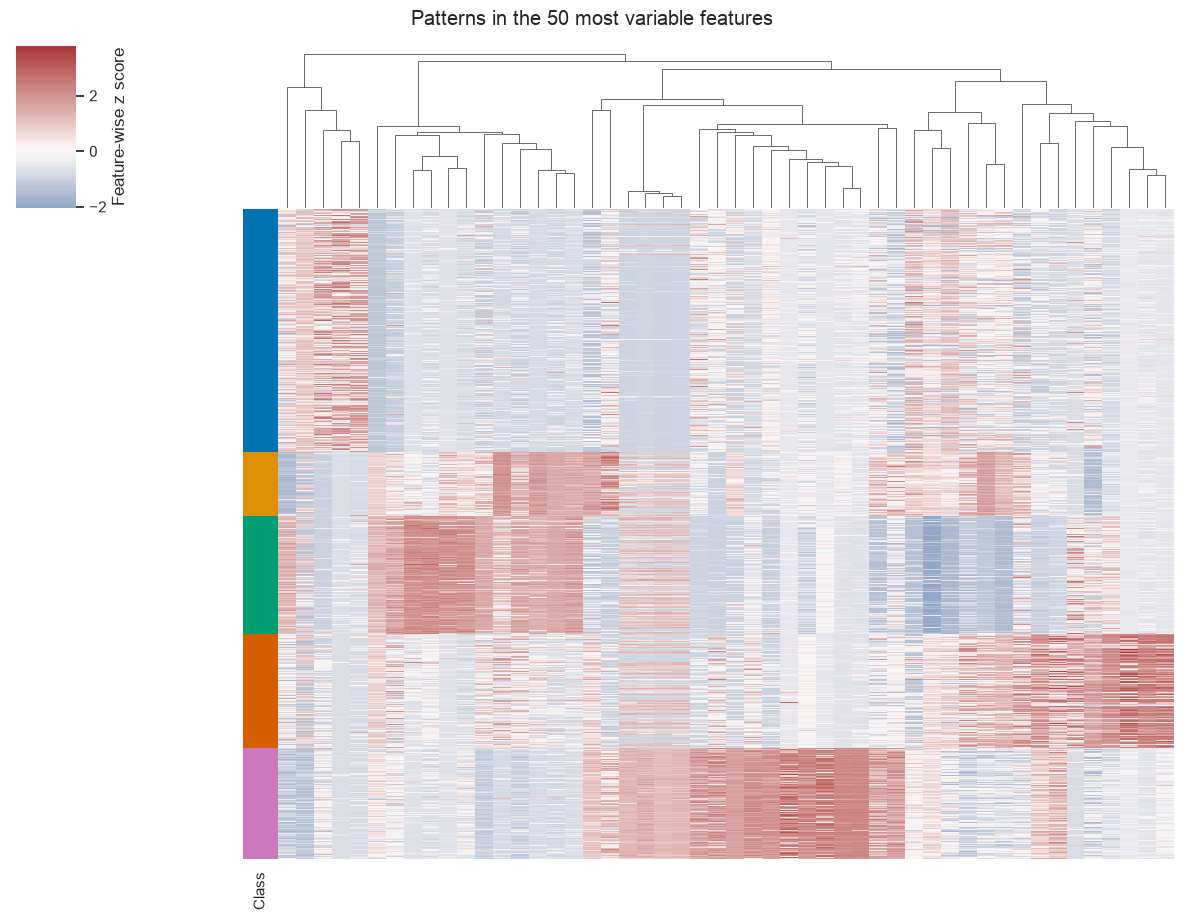
\includegraphics[width=\linewidth,height=0.39\textheight,keepaspectratio]{figures/06_top_variable_feature_heatmap.png}
  \end{column}

  \begin{column}{0.41\textwidth}
    {\condheading\bfseries\small\textcolor{navy}{Pattern Observations}}\par\vspace{2pt}
    \begin{itemize}\itemsep=2pt \scriptsize
      \item \textbf{Top 50 Variable Genes}: Standardized relative expression across all 801 patients.
      \item \textbf{Block-Diagonal Structure}: Distinct expression signatures align clearly with cancer cohorts (BRCA, KIRC, COAD, LUAD, PRAD).
      \item \textbf{Hierarchical Dendrogram}: Patient samples cluster predominantly by tissue origin.
      \item \textbf{Collinear Blocks}: Correlated gene blocks reflect co-regulated biological pathways.
    \end{itemize}
  \end{column}
\end{columns}

\takeaway{Natural clustering validates that the dataset contains strong class-specific signals, motivating linear classification.}
\end{frame}

% ==============================================================================
% SLIDE 6: PCA 2D PROJECTION (Two-Column Figure + Interpretation)
% ==============================================================================
\begin{frame}
\frametitle{Principal Component Analysis: 2D Unsupervised Projection}
\framesubtitle{Spectral decomposition confirms natural separability in orthogonal space}

\begin{columns}[c]
  \begin{column}{0.57\textwidth}
    \centering
    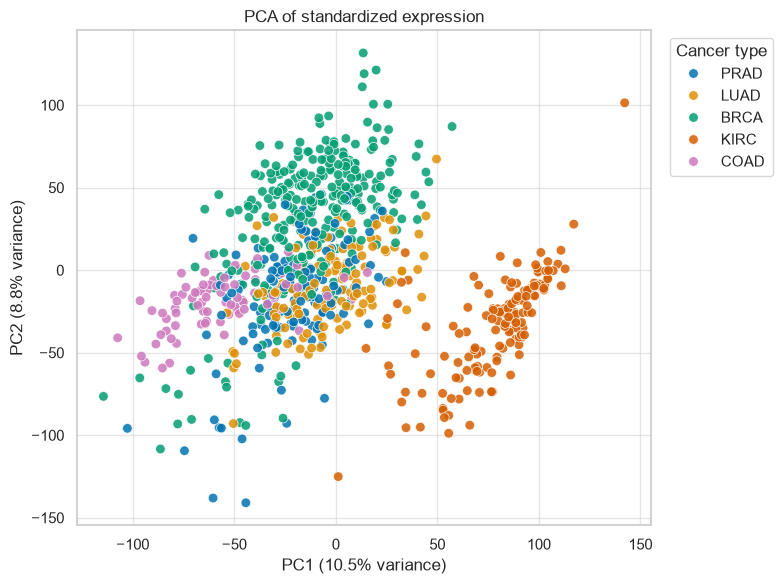
\includegraphics[width=\linewidth,height=0.39\textheight,keepaspectratio]{figures/05_pca_pc1_pc2.png}
  \end{column}

  \begin{column}{0.41\textwidth}
    {\condheading\bfseries\small\textcolor{navy}{Variance Decomposition}}\par\vspace{2pt}
    \begin{itemize}\itemsep=2pt \scriptsize
      \item \textbf{PC1 (18.6\% variance)}: Separates breast carcinoma (BRCA) cleanly from kidney renal clear cell (KIRC).
      \item \textbf{PC2 (12.3\% variance)}: Distinguishes colon adenocarcinoma (COAD) and lung (LUAD).
      \item \textbf{Cumulative Variance}: \textbf{30.9\%} of total variation captured in just two linear dimensions.
      \item \textbf{Cluster Separation}: Cohorts form distinct clusters without non-linear transformations.
    \end{itemize}
  \end{column}
\end{columns}

\takeaway{The 5 tumor types are largely linearly separable in an unsupervised 2D projection, bounding the need for complex classifiers.}
\end{frame}

% ==============================================================================
% SECTION 02: STATISTICAL METHODOLOGY
% ==============================================================================
\sectiondivider{02}{Statistical Methodology}{Regularized multinomial regression, tree ensembles, and neural baselines}

% ==============================================================================
% SLIDE 8: REGULARIZED LINEAR MODELS (Three-Column Comparative)
% ==============================================================================
\begin{frame}
\frametitle{Regularized Linear Models: Ridge, Lasso, and Elastic Net}
\framesubtitle{Controlling ill-conditioned multinomial cross-entropy in $p \gg n$}

\begin{columns}[T]
  \begin{column}{0.31\textwidth}
    \begin{panel}[Ridge ($L_2$ Regularization)]
      {\scriptsize $$\min_{\mathbf{W}} \mathcal{L}_{\text{CE}} + \frac{\lambda}{2}\sum_k \|\mathbf{w}_k\|_2^2$$}
      \begin{itemize}\itemsep=1.5pt
        \item Strictly convex Hessian ($\lambda \mathbf{I}$).
        \item Smooth weight shrinkage.
        \item Retains all \textbf{1,000 features}.
        \item Optimal probability calibration.
      \end{itemize}
    \end{panel}
  \end{column}

  \begin{column}{0.31\textwidth}
    \begin{panel}[Lasso ($L_1$ Regularization)]
      {\scriptsize $$\min_{\mathbf{W}} \mathcal{L}_{\text{CE}} + \lambda\sum_k \|\mathbf{w}_k\|_1$$}
      \begin{itemize}\itemsep=1.5pt
        \item Polyhedral $L_1$ geometry.
        \item Highly sparse: \textbf{89 active genes}.
        \item \textcolor{coral}{\textbf{Limitation:}} Arbitrarily selects 1 gene from collinear clusters.
      \end{itemize}
    \end{panel}
  \end{column}

  \begin{column}{0.31\textwidth}
    \begin{panel}[Elastic Net ($L_1 + L_2$)]
      {\tiny $$\min_{\mathbf{W}} \mathcal{L}_{\text{CE}} + \lambda\sum_k \left[\alpha \|\mathbf{w}_k\|_1 + \tfrac{1-\alpha}{2}\|\mathbf{w}_k\|_2^2\right]$$}
      \begin{itemize}\itemsep=1.5pt
        \item Sparsity + stability ($\alpha = 0.5$).
        \item Selects \textbf{218 active genes}.
        \item \textcolor{teal}{\textbf{Grouping property:}} Retains co-regulated pathway genes.
      \end{itemize}
    \end{panel}
  \end{column}
\end{columns}

\takeaway{Regularization prevents weight divergence on separable data; Elastic Net addresses collinear feature selection directly.}
\end{frame}

% ==============================================================================
% SLIDE 9: GROUPING THEOREM & NON-LINEAR BASELINES (Two-Column Comparative)
% ==============================================================================
\begin{frame}
\frametitle{The Grouping Effect and Non-Linear Baselines}
\framesubtitle{Theoretical bound under collinearity and comparison against tree / neural models}

\begin{columns}[T]
  \begin{column}{0.48\textwidth}
    \begin{panel}[Elastic Net Grouping Property Theorem]
      For two standardized features $\mathbf{x}_i, \mathbf{x}_j$ with sample correlation $r$:
      $$|\hat{w}_i - \hat{w}_j| \le \frac{\sqrt{2(1 - r)}}{\lambda (1 - \alpha)} \|\mathbf{y}\|_2$$
      \begin{itemize}\itemsep=3pt
        \item As correlation $r \to 1$, coefficient difference bound $|\hat{w}_i - \hat{w}_j| \to 0$.
        \item Strongly correlated genes enter or leave the active set together.
        \item Resolves Lasso's arbitrary feature dropping across biological pathways.
      \end{itemize}
    \end{panel}
  \end{column}

  \begin{column}{0.48\textwidth}
    \begin{panel}[Non-Linear Baseline Architectures]
      \textbf{Tree Ensembles:}
      \begin{itemize}\itemsep=2.5pt
        \item \textbf{Random Forest}: 200 bagged trees, feature subsampling $m = \lfloor\sqrt{p}\rfloor \approx 31$.
        \item \textbf{XGBoost}: Gradient boosting ($\eta = 0.10$, max depth 4, 100 rounds).
      \end{itemize}
      \vspace{3pt}
      \textbf{Neural Networks:}
      \begin{itemize}\itemsep=2.5pt
        \item \textbf{PCA-MLP}: 434 PCs ($95\%$ variance) $\to 128 \to 64 \to 5$.
        \item \textbf{Sparse NN}: Input group-lasso penalty $\lambda \sum \|\mathbf{W}^{(1)}_{:,j}\|_2$.
      \end{itemize}
    \end{panel}
  \end{column}
\end{columns}

\takeaway{Elastic Net guarantees coefficient grouping for correlated genes, whereas greedy tree splits choose arbitrarily.}
\end{frame}

% ==============================================================================
% SECTION 03: EXPERIMENTAL DESIGN
% ==============================================================================
\sectiondivider{03}{Experimental Design}{Strict validation protocol, stability metrics, and stress tests}

% ==============================================================================
% SLIDE 11: EXPERIMENTAL PIPELINE (Horizontal Methodology Flowchart)
% ==============================================================================
\begin{frame}
\frametitle{Experimental Pipeline: Zero-Leakage Validation}
\framesubtitle{Strict nested evaluation protocol across 10 independent stratified splits}

\vspace{0.05cm}
\begin{center}
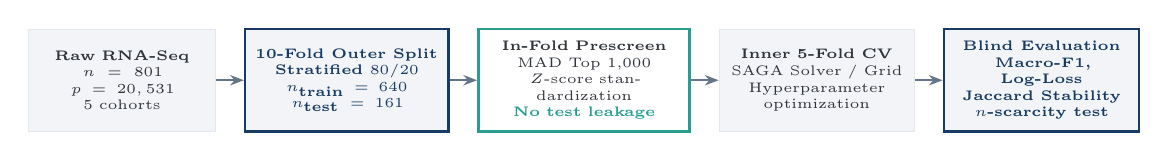
\begin{tikzpicture}[
  node distance=0.35cm,
  box/.style={draw=linegrey, fill=lightgrey, text=charcoal, font=\tiny, align=center, inner sep=4pt, minimum height=1.3cm},
  accentbox/.style={draw=teal, fill=white, text=charcoal, font=\tiny, align=center, inner sep=4pt, minimum height=1.3cm, line width=1.0pt},
  navybox/.style={draw=navy, fill=lightgrey, text=navy, font=\tiny\bfseries, align=center, inner sep=4pt, minimum height=1.3cm, line width=0.9pt},
  arr/.style={-{Stealth[scale=0.7]}, draw=mutedgrey, line width=0.9pt}
]
  \node[box, text width=2.1cm] (raw) {\textbf{Raw RNA-Seq}\\$n = 801$\\$p = 20,531$\\5 cohorts};
  \node[navybox, right=of raw, text width=2.3cm] (split) {\textbf{10-Fold Outer Split}\\Stratified $80/20$\\$n_{\text{train}} = 640$\\$n_{\text{test}} = 161$};
  \node[accentbox, right=of split, text width=2.4cm] (screen) {\textbf{In-Fold Prescreen}\\MAD Top 1,000\\$Z$-score standardization\\\textcolor{teal}{\textbf{No test leakage}}};
  \node[box, right=of screen, text width=2.2cm] (tune) {\textbf{Inner 5-Fold CV}\\SAGA Solver / Grid\\Hyperparameter\\optimization};
  \node[navybox, right=of tune, text width=2.2cm] (eval) {\textbf{Blind Evaluation}\\Macro-F1, Log-Loss\\Jaccard Stability\\$n$-scarcity test};

  \draw[arr] (raw) -- (split);
  \draw[arr] (split) -- (screen);
  \draw[arr] (screen) -- (tune);
  \draw[arr] (tune) -- (eval);
\end{tikzpicture}
\end{center}

\vspace{0.05cm}
\begin{columns}[T]
  \begin{column}{0.48\textwidth}
    \begin{panel}[Strict Test Set Isolation]
      \scriptsize Feature screening and standardization parameters ($\mu, \sigma$) are computed solely on training folds; test folds remain completely blind until final evaluation.
    \end{panel}
  \end{column}
  \begin{column}{0.48\textwidth}
    \begin{panel}[Repeated Outer Splits]
      \scriptsize 10 independent random resamplings quantify performance variance, feature selection stability, and model robustness under varied sample draws.
    \end{panel}
  \end{column}
\end{columns}

\takeaway{Nested protocol ensures that neither feature screening nor parameter scaling leaks test set information.}
\end{frame}

% ==============================================================================
% SLIDE 12: MULTI-CRITERIA METRICS (Three-Column Explanatory)
% ==============================================================================
\begin{frame}
\frametitle{Multi-Criteria Evaluation: Beyond Classification Accuracy}
\framesubtitle{Evaluating discrimination, probabilistic calibration, and biomarker stability}

\begin{columns}[T]
  \begin{column}{0.31\textwidth}
    \begin{panel}[Macro-F1 Score]
      {\scriptsize $$\text{Macro-F1} = \frac{1}{K}\sum_{k=1}^5 \frac{2 P_k R_k}{P_k + R_k}$$}
      \begin{itemize}\itemsep=1.5pt
        \item Unweighted class mean.
        \item Prevents BRCA ($n=300$) from masking COAD ($n=78$).
      \end{itemize}
    \end{panel}
  \end{column}

  \begin{column}{0.31\textwidth}
    \begin{panel}[Multi-Class Log-Loss]
      {\scriptsize $$\mathcal{L}_{\text{log}} = -\frac{1}{N}\sum_{i, k} y_{ik}\log(\hat{p}_{ik})$$}
      \begin{itemize}\itemsep=1.5pt
        \item Tests probability calibration.
        \item Penalizes overconfident wrong assignments.
      \end{itemize}
    \end{panel}
  \end{column}

  \begin{column}{0.31\textwidth}
    \begin{panel}[Selection Stability]
      {\scriptsize $$D = \frac{2|S_a \cap S_b|}{|S_a| + |S_b|}, \; J = \frac{|S_a \cap S_b|}{|S_a \cup S_b|}$$}
      \begin{itemize}\itemsep=1.5pt
        \item Pairwise split overlap.
        \item Quantifies biomarker reproducibility.
      \end{itemize}
    \end{panel}
  \end{column}
\end{columns}

\takeaway{In linearly separable settings, accuracy saturates; log-loss and stability expose genuine model quality.}
\end{frame}

% ==============================================================================
% SECTION 04: RESULTS AND COMPARISON
% ==============================================================================
\sectiondivider{04}{Results and Comparison}{Macro-F1 saturation, probability calibration, and the Pareto frontier}

% ==============================================================================
% SLIDE 14: BENCHMARK BOXPLOTS (Two-Column Figure + Analysis)
% ==============================================================================
\begin{frame}
\frametitle{Benchmark Performance Across 10 Repeated Splits}
\framesubtitle{Macro-F1 saturation vs.\ prominent divergence in probabilistic log-loss}

\begin{columns}[c]
  \begin{column}{0.60\textwidth}
    \centering
    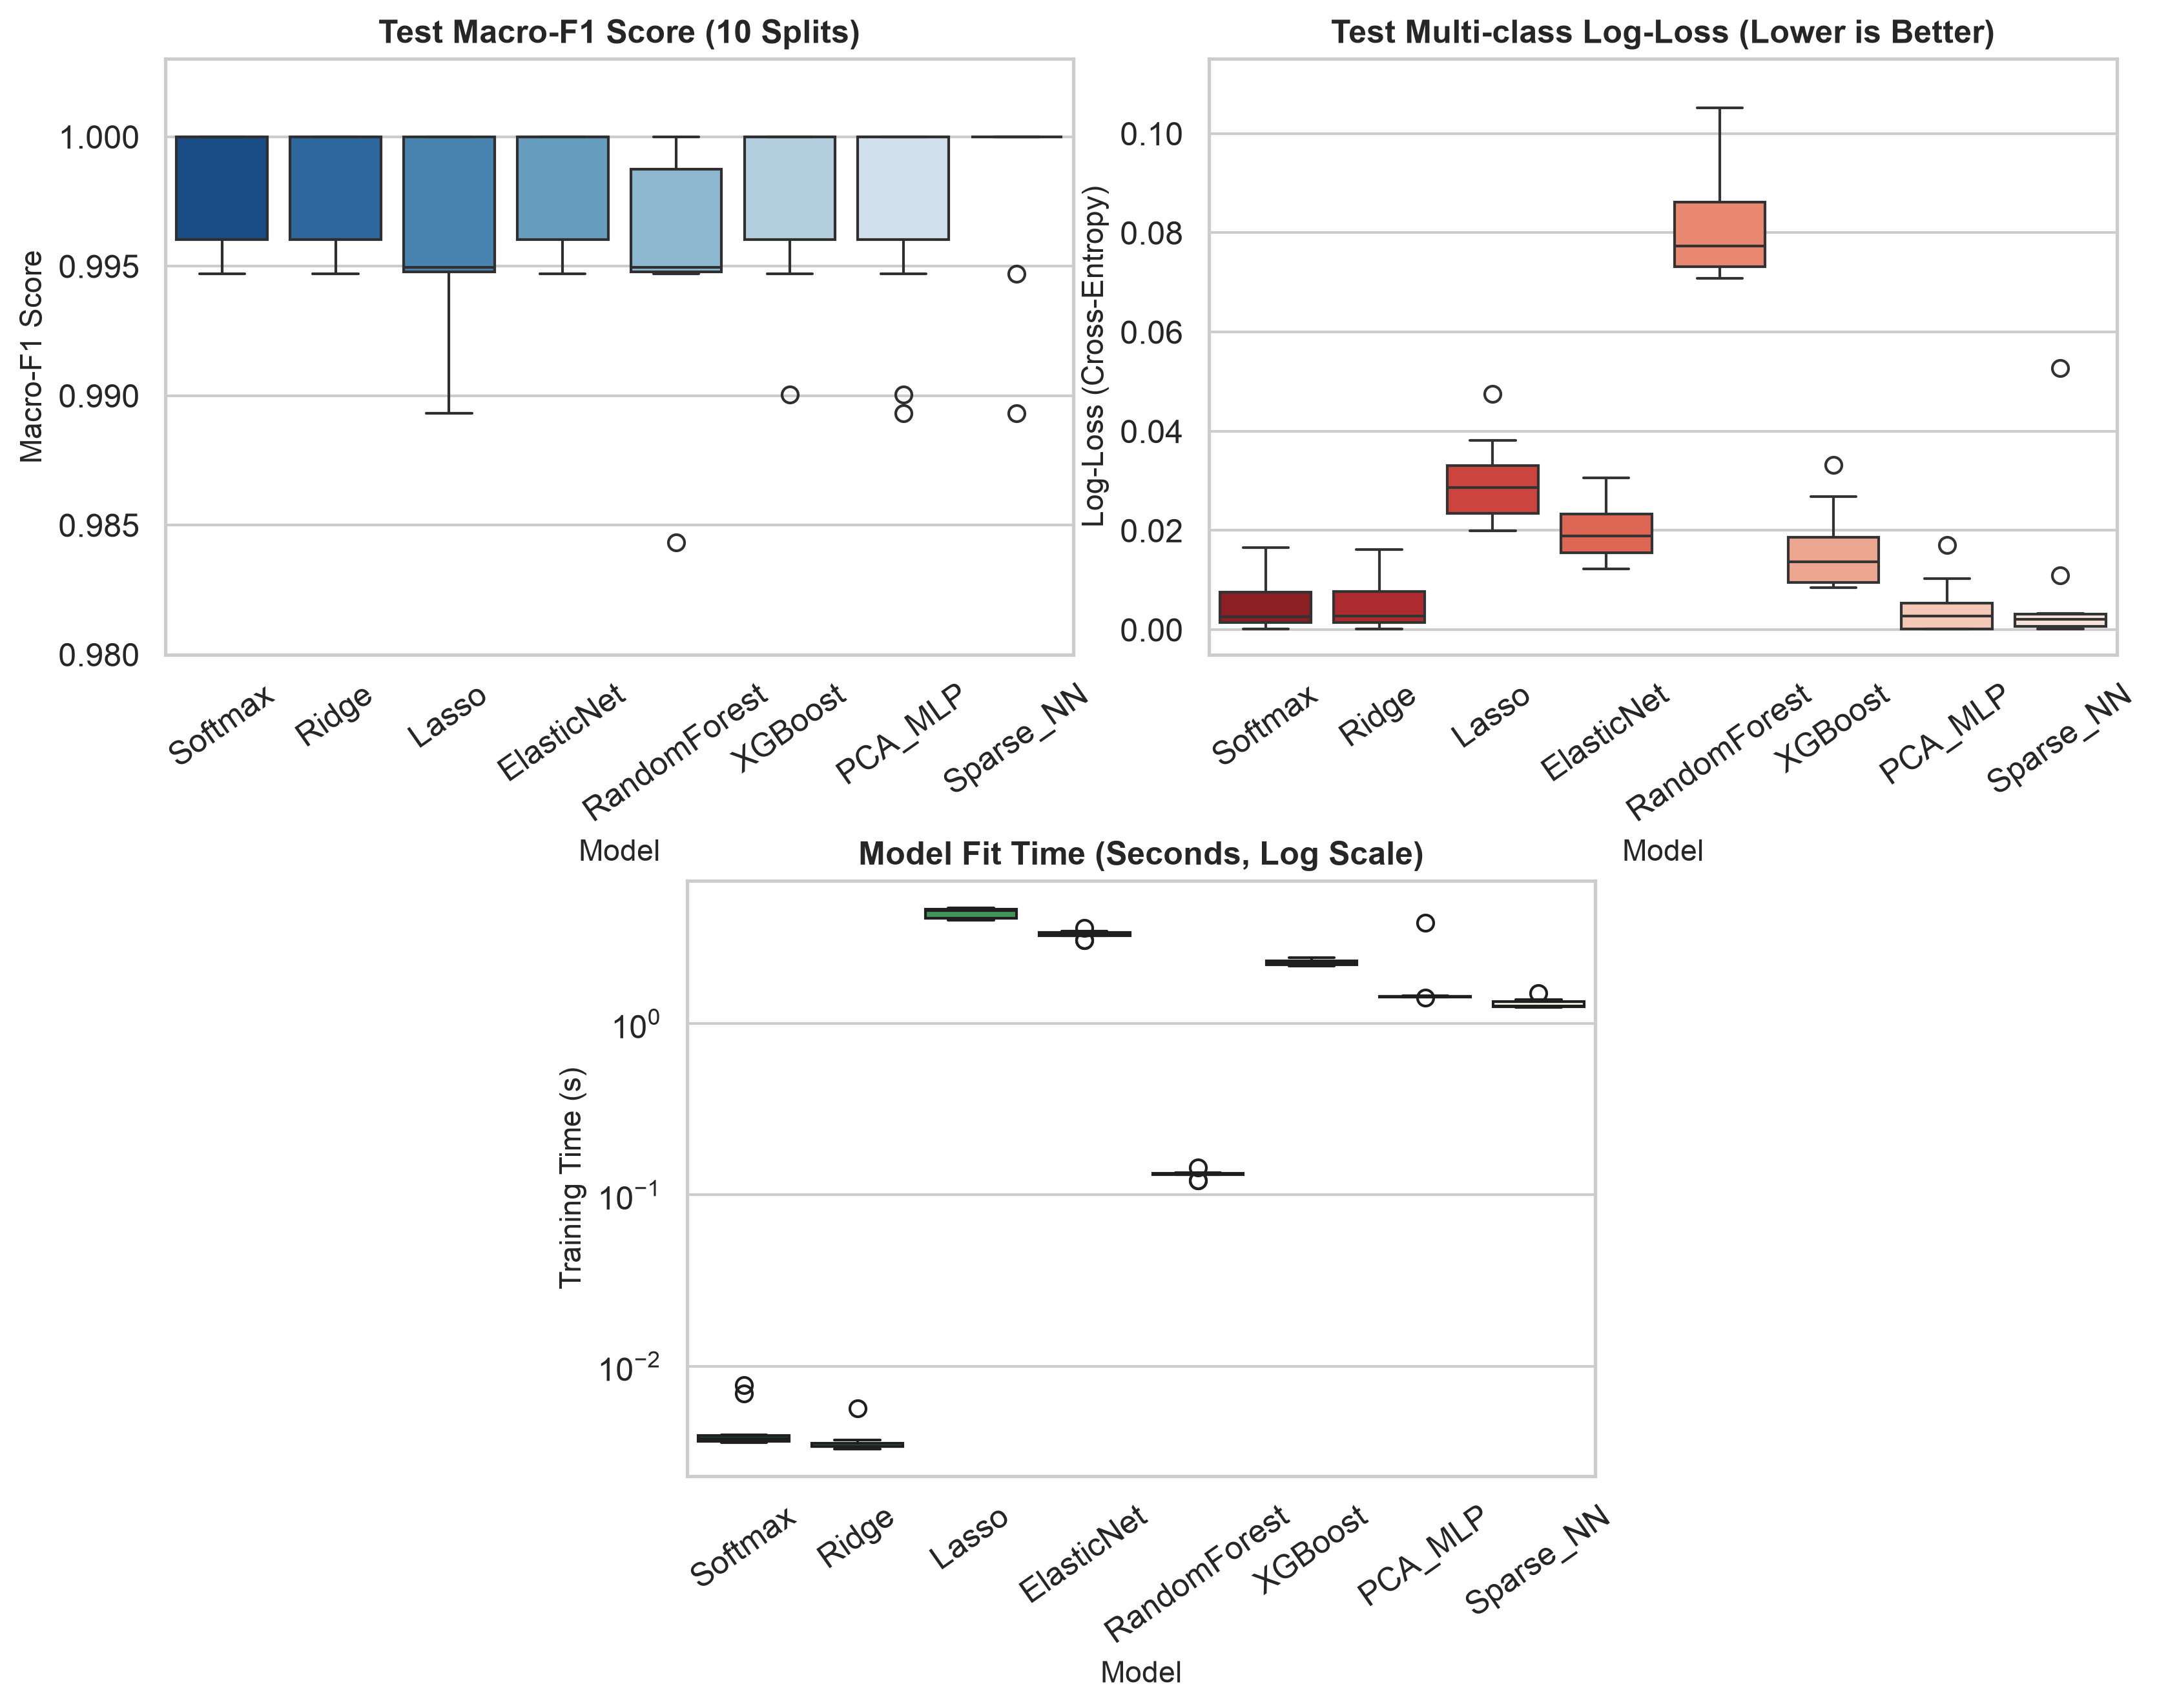
\includegraphics[width=\linewidth,height=0.39\textheight,keepaspectratio]{figures/01_model_comparison_boxplots.png}
  \end{column}

  \begin{column}{0.38\textwidth}
    {\condheading\bfseries\small\textcolor{navy}{Quantitative Breakdown}}\par\vspace{2pt}
    \begin{itemize}\itemsep=2pt \scriptsize
      \item \textbf{Macro-F1 Saturation}: All 8 models achieve mean Macro-F1 $\ge 0.993$. Accuracy alone cannot rank these architectures.
      \item \textbf{Log-Loss Divergence}:
        \begin{itemize}\itemsep=2pt
          \item Linear models and PCA-MLP achieve $< 0.020$ log-loss (sharp calibration).
          \item Random Forest exhibits \textbf{$0.081$ log-loss} due to probability softening from vote averaging.
          \item Sparse NN yields \textbf{$0.063$ log-loss}.
        \end{itemize}
    \end{itemize}
  \end{column}
\end{columns}

\takeaway{Multi-class log-loss reveals calibration deficits in tree ensembles that are invisible in accuracy metrics.}
\end{frame}

% ==============================================================================
% SLIDE 15: COMPREHENSIVE BENCHMARK TABLE (Large Comparison Table)
% ==============================================================================
\begin{frame}
\frametitle{Comprehensive Model Comparison Table}
\framesubtitle{Evaluation across discrimination, calibration, active sparsity, and runtime}

\vspace{0.05cm}
\centering
\footnotesize
\begin{tabular}{lccccc}
  \toprule
  \textbf{Model} & \textbf{Macro-F1} & \textbf{Log-Loss} & \textbf{Active Features} & \textbf{Fit Time (s)} & \textbf{Stability ($D$ / $J$)} \\
  \midrule
  \textbf{Softmax} & $0.998 \pm 0.003$ & $0.005 \pm 0.002$ & $1,000$ & $0.004$ & $1.000$ / $1.000$ \\
  \textbf{Ridge ($L_2$)} & $0.998 \pm 0.003$ & $0.005 \pm 0.002$ & $1,000$ & $0.004$ & $1.000$ / $1.000$ \\
  \textbf{Lasso ($L_1$)} & $0.995 \pm 0.006$ & $0.030 \pm 0.015$ & \textbf{89} & $4.44$ & $0.609$ / $0.443$ \\
  \rowcolor{lightgrey}
  \textbf{\textcolor{navy}{Elastic Net}} & \textbf{0.998} $\pm 0.003$ & $0.020 \pm 0.007$ & \textbf{218} & $3.65$ & \textbf{0.725} / \textbf{0.573} \\
  \textbf{Random Forest} & $0.994 \pm 0.006$ & $0.081 \pm 0.010$ & $1,000$ & $0.13$ & $0.276$ / $0.160$ \\
  \textbf{XGBoost} & $0.995 \pm 0.006$ & $0.028 \pm 0.009$ & $1,000$ & $2.18$ & $0.443$ / $0.285$ \\
  \textbf{PCA-MLP} & $0.998 \pm 0.003$ & \textbf{0.004} $\pm 0.001$ & $434$ & $1.68$ & N/A \\
  \textbf{Sparse NN} & $0.997 \pm 0.004$ & $0.063 \pm 0.015$ & $1,000$ & $1.25$ & N/A \\
  \bottomrule
\end{tabular}

\vspace{0.15cm}
\takeaway{Elastic Net matches the top F1 score ($0.998$) while eliminating 78\% of candidate genes, outperforming trees in stability and calibration.}
\end{frame}

% ==============================================================================
% SLIDE 16: PARETO FRONTIER (Two-Column Figure + Trade-off Analysis)
% ==============================================================================
\begin{frame}
\frametitle{Active Feature Sparsity vs.\ Log-Loss: The Pareto Frontier}
\framesubtitle{Evaluating the direct trade-off between model parsimony and probability calibration}

\begin{columns}[c]
  \begin{column}{0.57\textwidth}
    \centering
    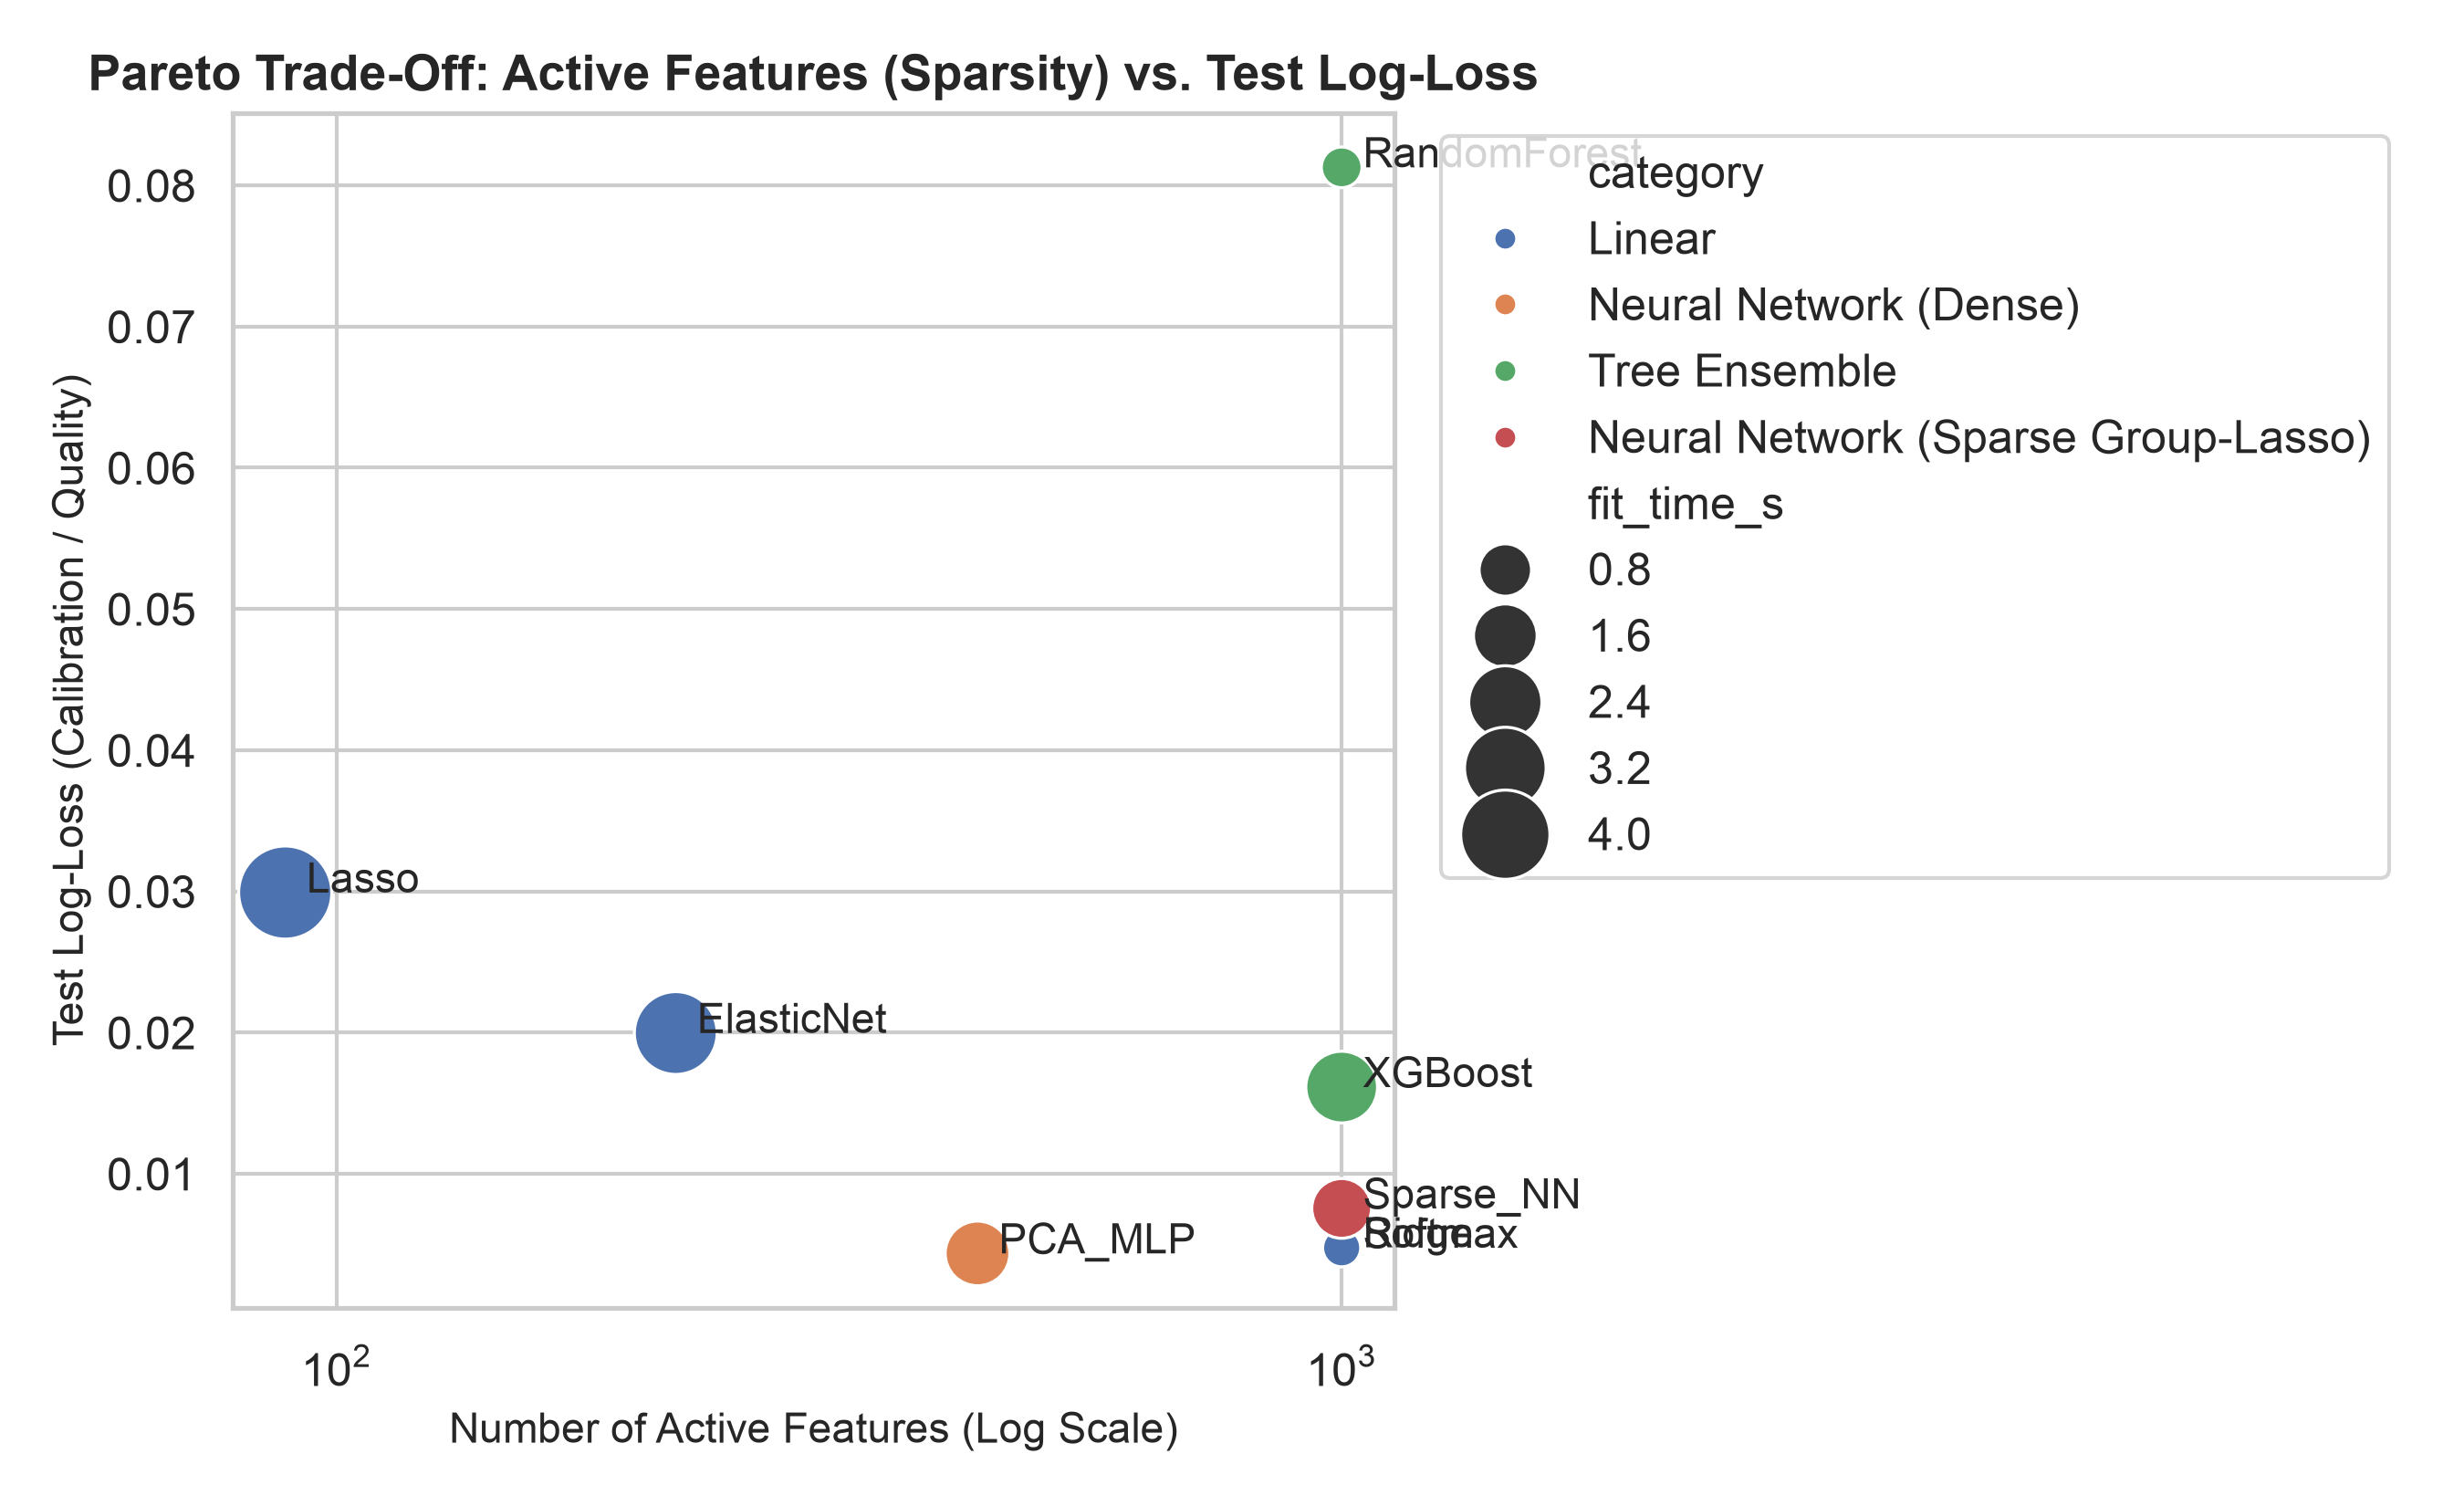
\includegraphics[width=\linewidth,height=0.39\textheight,keepaspectratio]{figures/05_pareto_frontier.png}
  \end{column}

  \begin{column}{0.41\textwidth}
    {\condheading\bfseries\small\textcolor{navy}{Trade-off Spectrum}}\par\vspace{2pt}
    \begin{itemize}\itemsep=2pt \scriptsize
      \item \textbf{Dense Boundary}: Ridge and PCA-MLP achieve minimal log-loss ($0.004\text{--}0.005$) by retaining all features or 434 principal components.
      \item \textbf{High Compression}: Lasso compresses to \textbf{89 active genes} with a modest log-loss trade-off ($0.030$).
      \item \textbf{The Optimal Compromise}: \textbf{Elastic Net} achieves $0.020$ log-loss with \textbf{218 genes}, balancing parsimony and calibration.
      \item \textbf{Tree Ensembles}: Fall far from the frontier due to softened probabilities.
    \end{itemize}
  \end{column}
\end{columns}

\takeaway{Elastic Net establishes the best compromise between biological interpretability and sharp test calibration.}
\end{frame}

% ==============================================================================
% SLIDE 17: FEATURE STABILITY (Two-Column Figure + Analysis)
% ==============================================================================
\begin{frame}
\frametitle{Feature Selection Stability across Resampling Splits}
\framesubtitle{Evaluating biomarker reproducibility under high pairwise collinearity}

\begin{columns}[c]
  \begin{column}{0.57\textwidth}
    \centering
    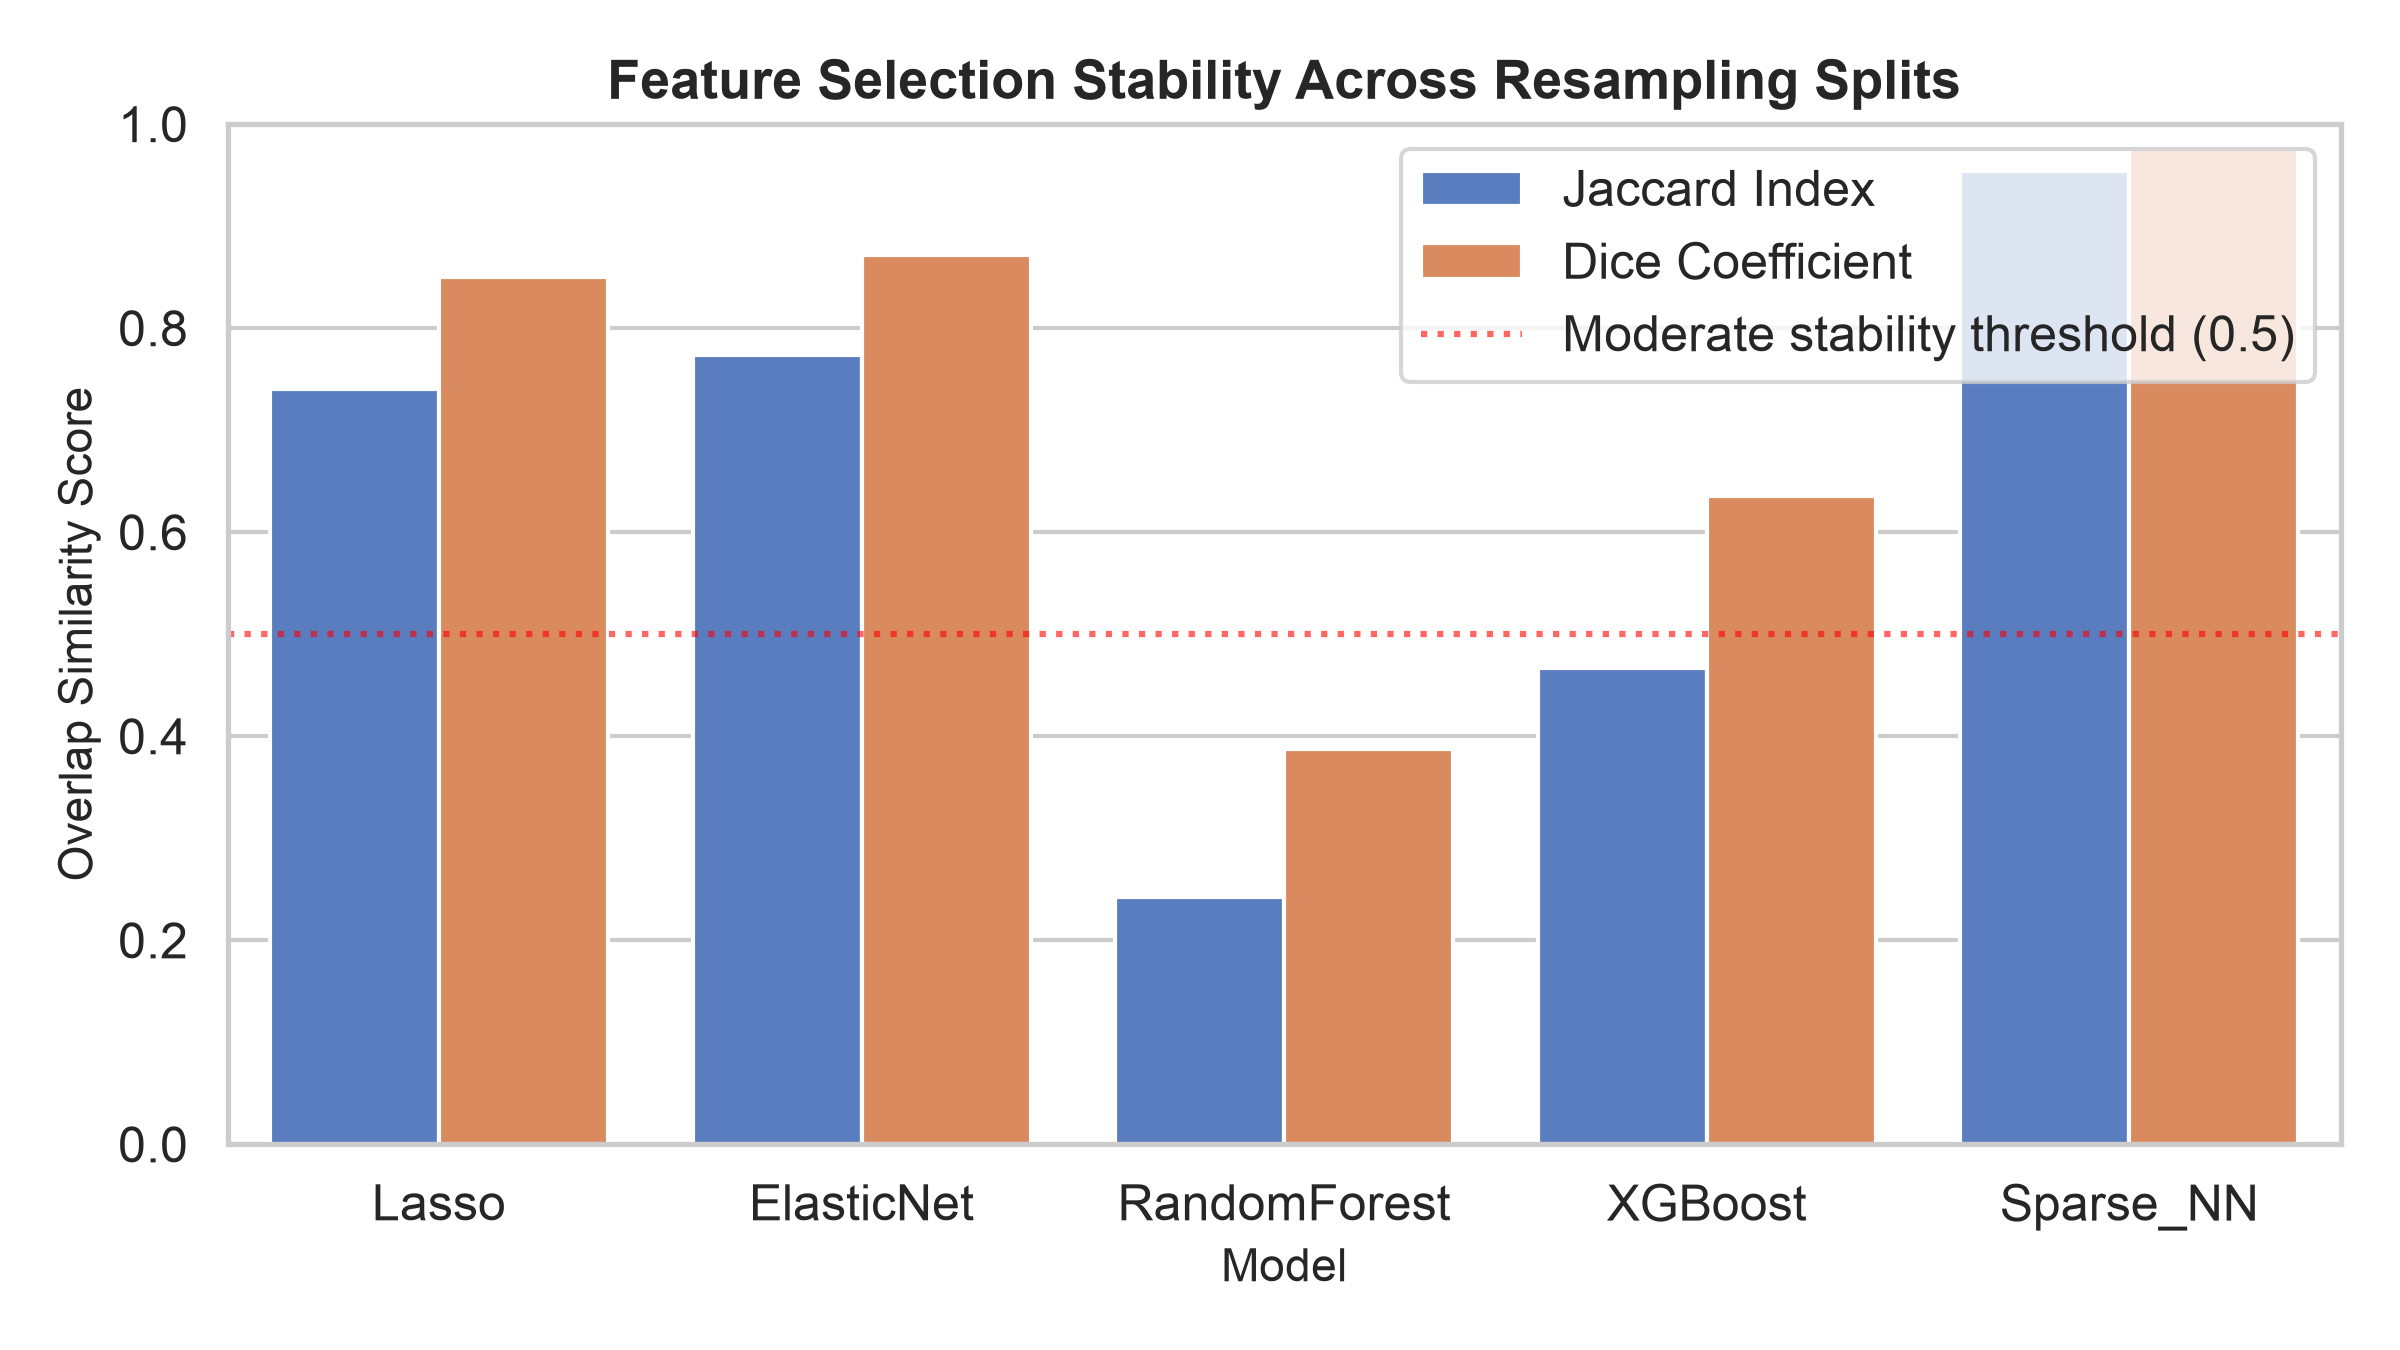
\includegraphics[width=\linewidth,height=0.39\textheight,keepaspectratio]{figures/04_feature_stability_barplot.png}
  \end{column}

  \begin{column}{0.41\textwidth}
    {\condheading\bfseries\small\textcolor{navy}{Stability Findings}}\par\vspace{2pt}
    \begin{itemize}\itemsep=2pt \scriptsize
      \item \textbf{Elastic Net Dominance}: Achieves top stability among sparse models (\textbf{Dice 0.725}, \textbf{Jaccard 0.573}) via $L_2$ grouping.
      \item \textbf{Lasso Degradation}: Moderate stability ($D=0.609$, $J=0.443$); randomly selects 1 feature from collinear groups.
      \item \textbf{Tree Split Collapse}: Random Forest ($J = 0.160$) and XGBoost ($J = 0.285$) show severe selection instability.
      \item \textbf{Mechanism}: Collinear features offer nearly identical impurity drops, causing tree splits to fluctuate randomly.
    \end{itemize}
  \end{column}
\end{columns}

\takeaway{Biomarker discovery requires $L_2$ regularization; greedy tree splitters cannot stably select correlated genes.}
\end{frame}

% ==============================================================================
% SLIDE 18: SAMPLE EFFICIENCY STRESS TEST (Two-Column Figure + Analysis)
% ==============================================================================
\begin{frame}
\frametitle{Sample Efficiency Stress Test: $n_{\text{train}} = 30 \to 640$}
\framesubtitle{Simulating extreme clinical sample scarcity down to 6 patients per cancer cohort}

\begin{columns}[c]
  \begin{column}{0.57\textwidth}
    \centering
    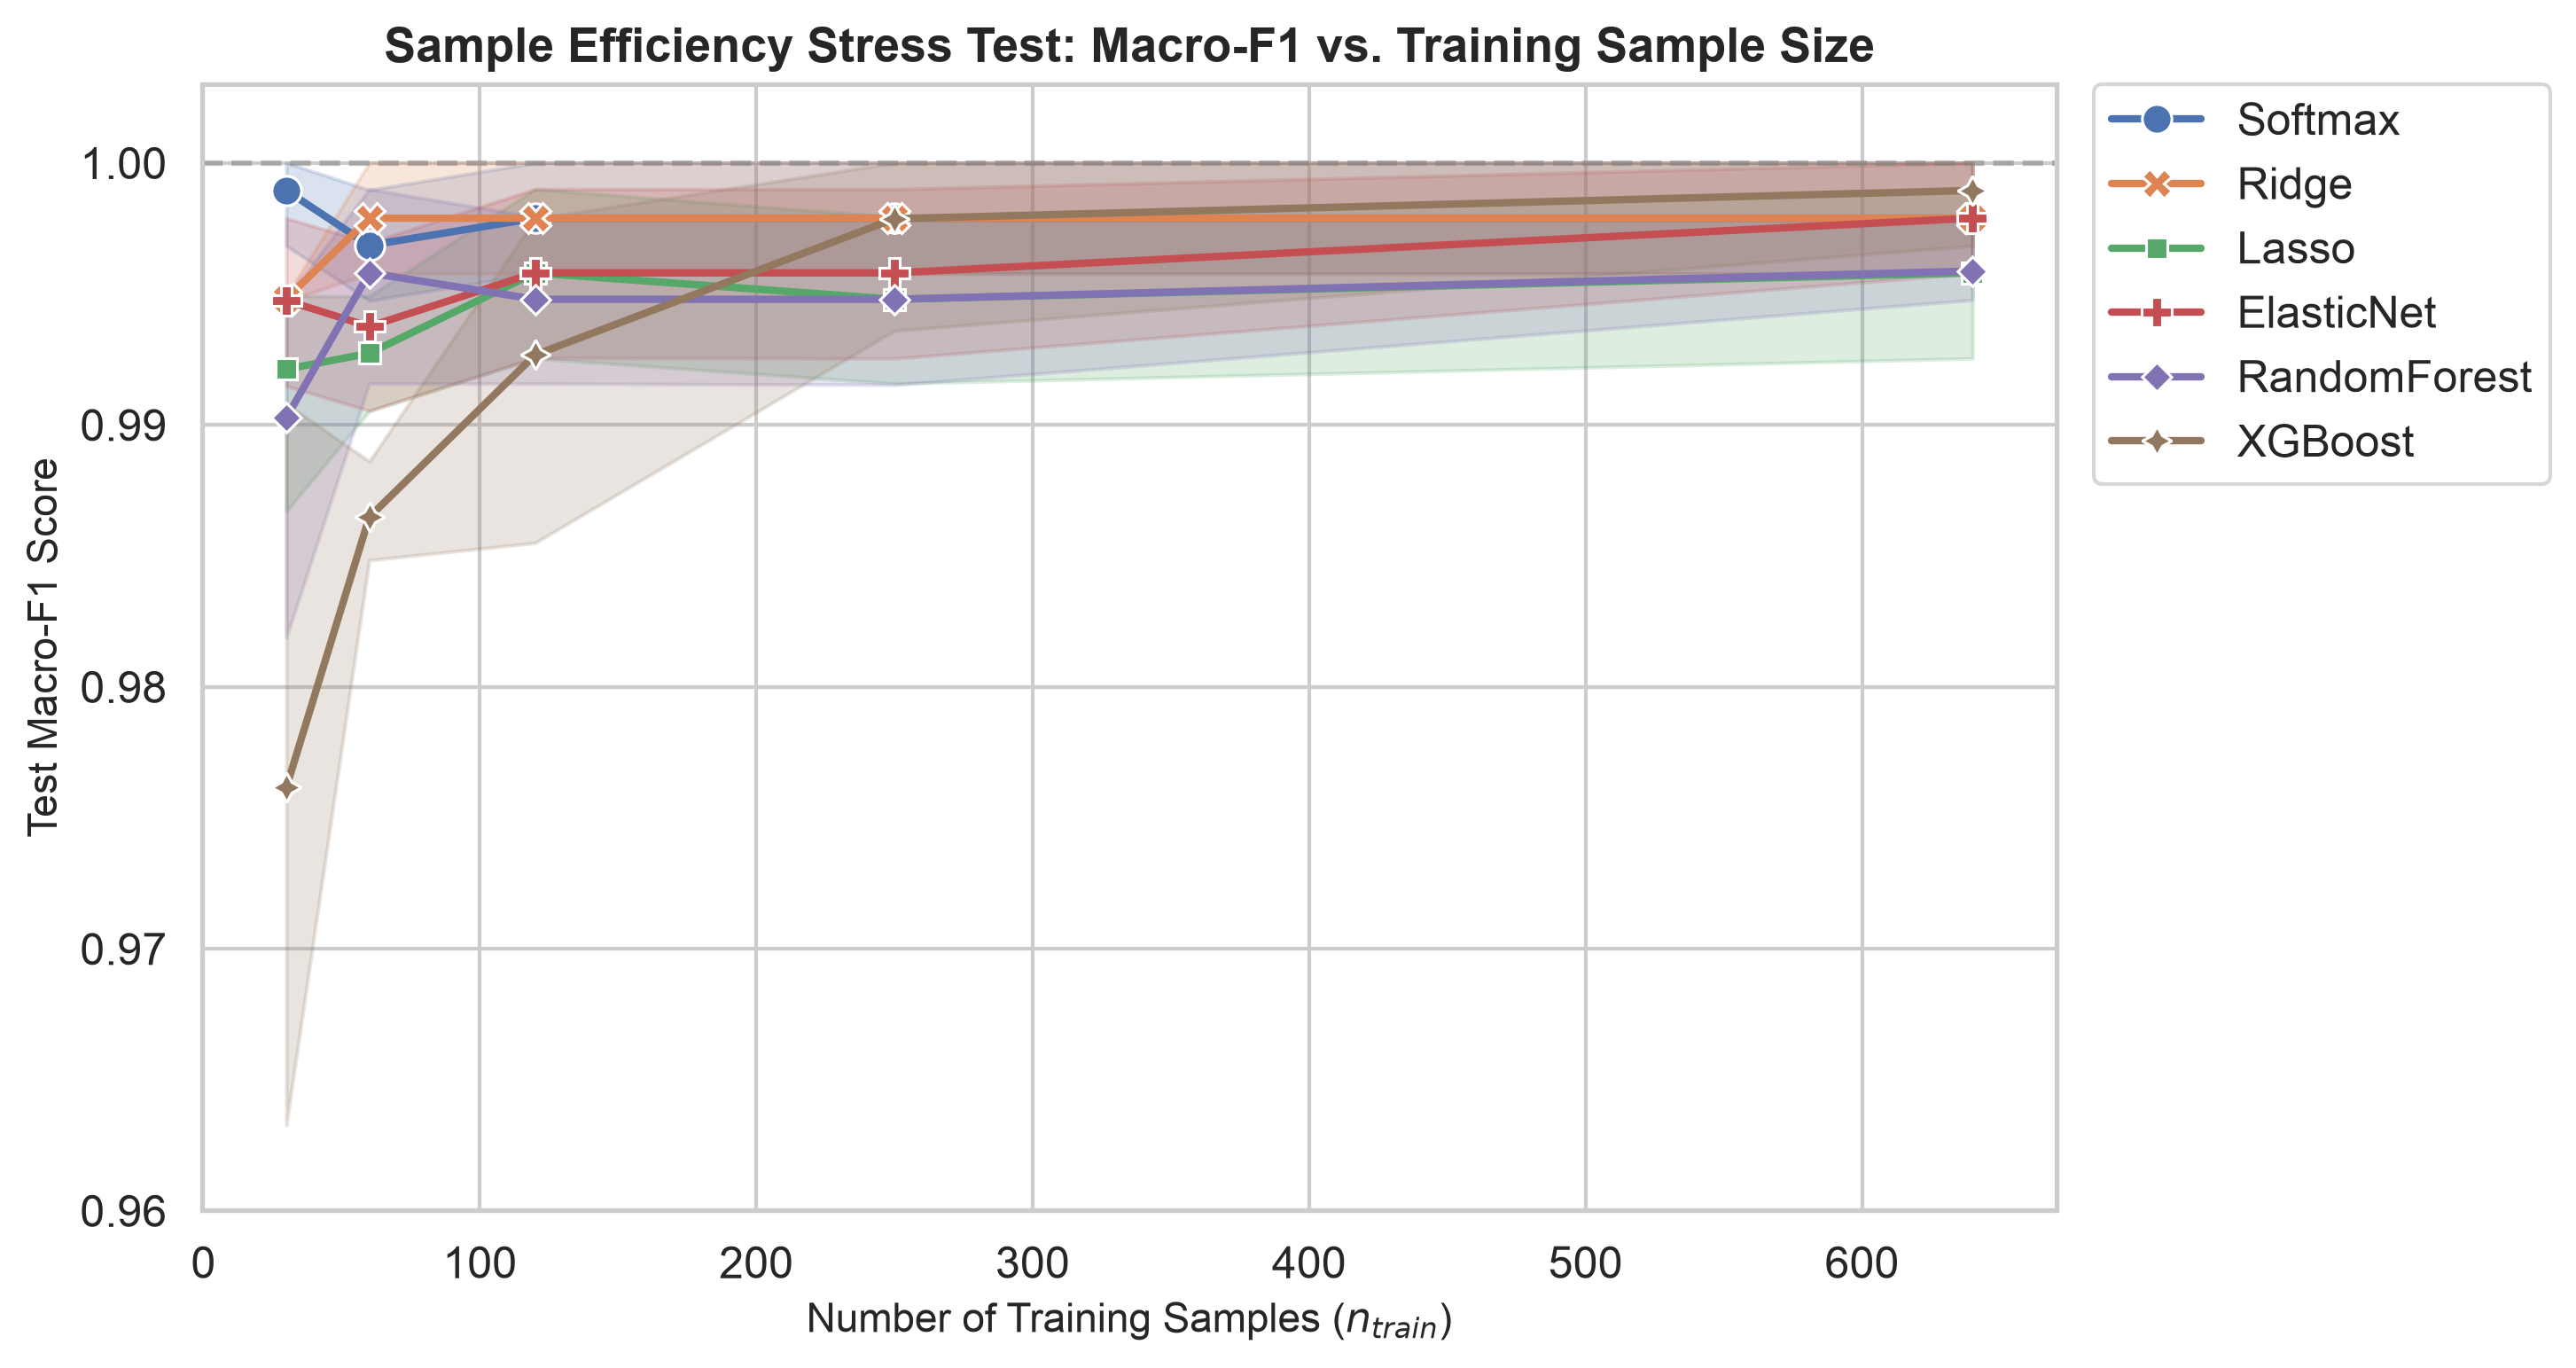
\includegraphics[width=\linewidth,height=0.39\textheight,keepaspectratio]{figures/02_n_efficiency_curves.png}
  \end{column}

  \begin{column}{0.41\textwidth}
    {\condheading\bfseries\small\textcolor{navy}{Scarcity Analysis}}\par\vspace{2pt}
    \begin{itemize}\itemsep=2pt \scriptsize
      \item \textbf{Linear Resilience}: Regularized linear models (Ridge, Softmax, Elastic Net) remain remarkably robust ($\ge \mathbf{0.995}$ Macro-F1) even at $n_{\text{train}} = 30$.
      \item \textbf{Tree Ensemble Drop}: XGBoost degrades to \textbf{$0.976 \pm 0.018$} (minimum fold score $0.954$). Random Forest drops to $0.985$.
      \item \textbf{Inductive Bias}: Strong linear assumptions protect against small-sample overfitting; non-linear step boundaries overfit when sample density is low.
    \end{itemize}
  \end{column}
\end{columns}

\takeaway{Regularized linear models exhibit superior sample efficiency, retaining high performance even under extreme sample scarcity.}
\end{frame}

% ==============================================================================
% SECTION 05: INTERPRETATION AND CONCLUSION
% ==============================================================================
\sectiondivider{05}{Interpretation and Conclusion}{Answers to research questions, limitations, and practical recommendations}

% ==============================================================================
% SLIDE 20: ANSWERS TO RESEARCH QUESTIONS (Three-Panel Structured Layout)
% ==============================================================================
\begin{frame}
\frametitle{Answers to Core Research Questions}
\framesubtitle{Synthesized conclusions from benchmark and stress-test experiments}

\begin{columns}[T]
  \begin{column}{0.31\textwidth}
    \begin{panel}[Q1. Flexibility in $p \gg n$?]
      \textbf{No Advantage.}
      \begin{itemize}\itemsep=1.5pt \scriptsize
        \item Linear separability means deep nets and boosting offer no accuracy gain over linear models.
        \item Non-linear models inflate calibration error.
      \end{itemize}
    \end{panel}
  \end{column}

  \begin{column}{0.31\textwidth}
    \begin{panel}[Q2. Collinearity Impact?]
      \textbf{Destabilizes Trees \& Lasso.}
      \begin{itemize}\itemsep=1.5pt \scriptsize
        \item Lasso arbitrarily drops pathway co-regulators.
        \item Trees suffer split instability ($J = 0.160$).
        \item Elastic Net $L_2$ grouping stabilizes selection ($J = 0.573$).
      \end{itemize}
    \end{panel}
  \end{column}

  \begin{column}{0.31\textwidth}
    \begin{panel}[Q3. Optimal Architecture?]
      \textbf{Elastic Net.}
      \begin{itemize}\itemsep=1.5pt \scriptsize
        \item Matches $0.998$ F1 with 78\% fewer genes (218 active).
        \item Balances calibration ($0.020$) and biomarker stability.
        \item Robust under sample scarcity ($n=30$).
      \end{itemize}
    \end{panel}
  \end{column}
\end{columns}

\takeaway{In high-dimensional transcriptomics, inductive bias and regularization dominate architectural complexity.}
\end{frame}

% ==============================================================================
% SLIDE 21: HONEST LIMITATIONS (Three-Column Editorial Layout)
% ==============================================================================
\begin{frame}
\frametitle{Honest Limitations and Methodological Scope}
\framesubtitle{Distinguishing benchmark findings from clinical translation requirements}

\begin{columns}[T]
  \begin{column}{0.31\textwidth}
    \begin{panel}[Single-Source Cohort]
      \begin{itemize}\itemsep=1.5pt \scriptsize
        \item Single TCGA batch ($n = 801$).
        \item Multi-center batch variations not assessed.
        \item Requires external prospective cohort validation.
      \end{itemize}
    \end{panel}
  \end{column}

  \begin{column}{0.31\textwidth}
    \begin{panel}[Primary vs.\ Fine Subtypes]
      \begin{itemize}\itemsep=1.5pt \scriptsize
        \item Primary tissue sites have large expression divergence.
        \item Intra-organ subtypes (e.g.\ breast luminal A vs.\ B) present subtle non-linear boundaries.
      \end{itemize}
    \end{panel}
  \end{column}

  \begin{column}{0.31\textwidth}
    \begin{panel}[Clinical Translation]
      \begin{itemize}\itemsep=1.5pt \scriptsize
        \item 218 genes form a computational screen for diagnostic assays.
        \item Candidates require biological assay validation before claiming causal biomarker status.
      \end{itemize}
    \end{panel}
  \end{column}
\end{columns}

\takeaway{Findings demonstrate strong linear separability for primary cancer types, while subtle subtyping remains an open question.}
\end{frame}

% ==============================================================================
% SLIDE 22: PRACTICAL RECOMMENDATIONS & CONCLUSION
% ==============================================================================
\begin{frame}
\frametitle{Summary and Practical Recommendations}
\framesubtitle{Key guidelines for practitioners analyzing high-dimensional RNA-Seq data}

\begin{columns}[T]
  \begin{column}{0.55\textwidth}
    {\condheading\bfseries\small\textcolor{navy}{Core Recommendations for Practitioners}}\par\vspace{2pt}
    \begin{itemize}\itemsep=2pt \scriptsize
      \item \textbf{Default to Elastic Net}: Use Elastic Net ($\alpha \approx 0.5$) as primary baseline; it combines high accuracy, 78\% sparsity, and grouping stability.
      \item \textbf{Avoid Unregularized Models}: Never fit standard OLS or LDA on $p \gg n$ data due to singular covariance.
      \item \textbf{Evaluate Beyond Accuracy}: Rely on multi-class log-loss and stability metrics to detect calibration loss and biomarker instability.
      \item \textbf{Exercise Caution with Trees}: Do not rely on tree split importance under high gene collinearity.
    \end{itemize}
  \end{column}

  \begin{column}{0.42\textwidth}
    \begin{panel}[Project Artifacts \& Code]
      \begin{itemize}\itemsep=1.5pt \scriptsize
        \item \textbf{Dataset}: 801 TCGA RNA-Seq samples ($K=5$).
        \item \textbf{Pipeline}: 10-fold nested CV with zero test leakage.
        \item \textbf{Report}: 10-page academic project paper with full derivations.
      \end{itemize}
      \vspace{2pt}
      \centering
      {\condheading\bfseries\small\textcolor{navy}{Thank You}}\;\textbar{}\;{\scriptsize\textcolor{mutedgrey}{Questions \& Discussion}}
    \end{panel}
  \end{column}
\end{columns}

\takeaway{Regularized linear models provide the most reliable, calibrated, and reproducible foundation for high-dimensional cancer classification.}
\end{frame}

\end{document}
